\section{Hardware/software mapping}
\textbf{Hardware/Software Mapping}\\
\begin{figure}[h!]
	\centering
		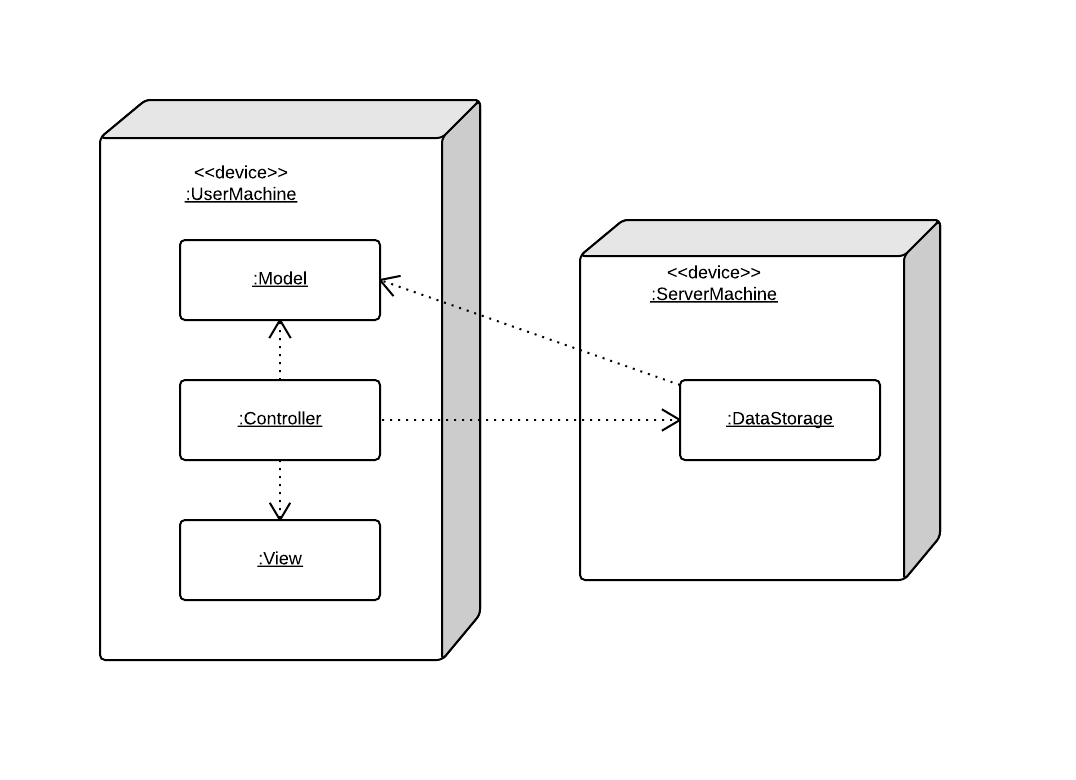
\includegraphics[scale=0.4]{HardwareSoftwareMapping}
	\caption{Zoom in to see details - Diagram of the Hardware/softwarem apping}
  \label{fig:HardwareSoftwareMapping}
\end{figure}\\\\
The three subsystems running on the UserMachine are Model, Controller and View. The Controller interacts both with the Model and the View, for logic and presentation. Upon saving an event in the CalendarSystem, the Controller will then communicate with the second device, the ServerMachine, and send/request data. Following this, the DataStorage returns the data to the Model and can be done with as pleased.